\section{New Bounded Acquisition: RQ4}
\label{sec:new_acquisition}
\subsection{Sampling, Timing and Observation Limits}
Before new requests, we froze 100 roots sampled without replacement from the original graph's 22,483 ordinary-shaped identifiers. This frame excludes bundled-context strings but remains inherited from the original seeded expansion. It is not a random sample of all npm. Latest root versions are frozen on retrieval; deps.dev supplies version-specific dependency observations, and version-specific npm requests supply fresh metadata and maintainer associations. No old workflow flags or dependency rows are copied into the new graph.

The bounded acquisition retains at most 500 nodes per root and 2,500 exact (package, version) nodes globally, prioritizing sampled roots and deterministic traversal. It obtains dependency graphs for 94 of the 100 roots; the six failures remain recorded and are not interpreted as empty dependency trees. None of the acquired graphs loses nodes to these caps. One acquired root contains 15 node-level API error records, which are retained rather than interpreted as complete resolution. The retained union has 1,641 exact nodes, 1,476 identifiers and 4,357 version-edge rows. All 1,641 ordinary version-metadata requests succeed. The 1,051 observed usernames are associations, without a historical authority interpretation.

Of 95 roots with parsed GitHub mappings, 89 yield a commit observation and 74 yield a directory listing at that pinned commit. Requiring both dependency acquisition and directory observation retains 70 root records, which map to 66 repository endpoints; 65 have an observed source. The acquired directory is still a presence proxy. Missing mappings, commit observations, and directory observations remain documented missingness rather than evidence of safety. Requests span a collection window rather than a shared instantaneous cutoff.

\subsection{Within-Cohort Tradeoffs and Representation}
% Generated by scripts/render_journal_validation.py
\begin{table*}[t]
\centering
\footnotesize
\caption{Budget-100 results in the newly acquired bounded cohort: 66 workflow-associated repositories, 65 with observed sources.}
\label{tab:revision_replication}
\begin{tabular}{llrrrr}
\toprule
Representation & Rule & $C$ & $C$ (\%) & $H$ (\%) & $P$\\
\midrule
Name & Portfolio & 41 & 62.12 & 13.51 & 6\\
Name & Exact union & 42 & 63.64 & 44.95 & 4\\
Name & Greedy coverage & 65 & 98.48 & 11.19 & 11\\
Name & Original direct P & 62 & 93.94 & 17.72 & 34\\
Name & Immediate + coverage & 63 & 95.45 & 14.23 & 28\\
Version & Portfolio & 41 & 62.12 & 13.44 & 6\\
Version & Exact union & 43 & 65.15 & 45.17 & 4\\
Version & Greedy coverage & 65 & 98.48 & 11.28 & 11\\
Version & Original direct P & 62 & 93.94 & 16.42 & 35\\
Version & Immediate + coverage & 63 & 95.45 & 13.48 & 29\\
\bottomrule
\end{tabular}
\par\smallskip\begin{minipage}{0.98\textwidth}\footnotesize The cohort has 1,051 observed accounts. H denominators are 2,494 name pairs and 2,411 version pairs. Root selection comes from the original ordinary-name frame; acquisition failures remain recorded and six missing dependency graphs are not treated as empty graphs.\end{minipage}
\end{table*}

At budget 100, greedy coverage reaches \ReplicationGreedyC{} of \ReplicationEndpoints{} endpoints, while exact union reaches \ReplicationUnionC{}. Their within-cohort H values are 11.19\% and 44.95\%. The original exclusion heuristic gives $P=34$, compared with greedy's 11 and union's four; the immediate-completion variant gives 28. Thus the simpler rule's slight original-graph advantage does not transport to this cohort.

\begin{figure*}[t]
\centering
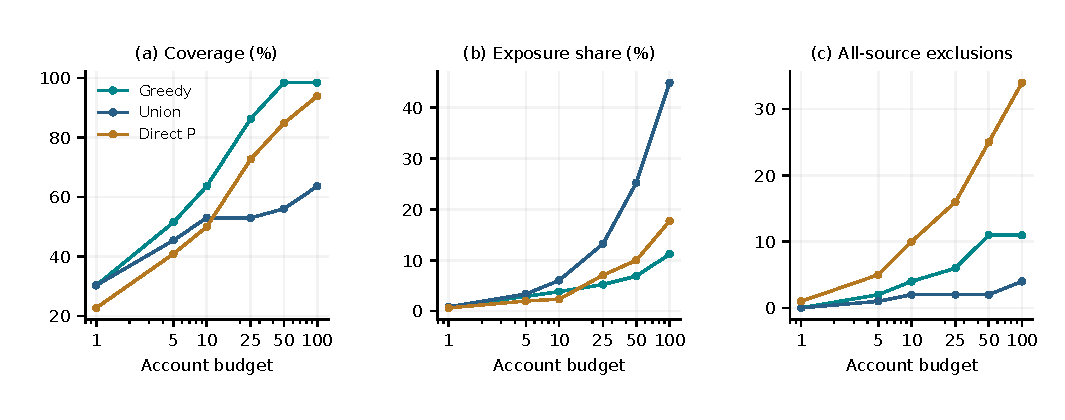
\includegraphics[width=0.98\textwidth]{revision_replication.pdf}
\caption{New-cohort name-graph comparisons across the six frozen budgets. Coverage uses 66 observed repository endpoints, H uses 2,494 account--repository pairs, and P excludes the source-free endpoint. Curves reuse one acquired cohort and supply no npm-wide uncertainty estimate.}
\label{fig:revision_replication}
\end{figure*}

Version continuity reduces pair mass from 2,494 to 2,411, a \ReplicationPairDecrease\% decrease. The original graph's 42.44\% decrease therefore does not describe a universal representation correction. The two acquisitions differ in roots, observed graph extent, versions and dates; their difference cannot be attributed solely to temporal change. The repeated coverage--exposure ordering is descriptive evidence of transport under these explicit observation conditions, not a measured intervention effect.

\subsection{Common Endpoints and Eligible Accounts}
% Generated by scripts/render_journal_validation.py
\begin{table*}[t]
\centering
\footnotesize
\caption{Reoptimized budget-100 selections on 65 common repository keys with 1,036 common selectable accounts.}
\label{tab:revision_common}
\begin{tabular}{llrrrr}
\toprule
Dataset & Rule & $C$ & $H$ (\%) & $P$ & Pair mass\\
\midrule
Original & Exact union & 52 & 21.55 & 4 & 12,833\\
Original & Greedy coverage & 65 & 6.09 & 8 & 12,833\\
Original & Original direct P & 65 & 11.72 & 20 & 12,833\\
New cohort & Exact union & 43 & 44.87 & 4 & 2,487\\
New cohort & Greedy coverage & 64 & 11.22 & 11 & 2,487\\
New cohort & Original direct P & 62 & 17.25 & 34 & 2,487\\
\bottomrule
\end{tabular}
\par\smallskip\begin{minipage}{0.98\textwidth}\footnotesize Complete source sets are preserved, including sources outside the common eligible account set. Pair denominators differ by observed graph, so H percentages are within-dataset quantities rather than a causal temporal effect.\end{minipage}
\end{table*}

We also reoptimize on 65 common repository keys with 1,036 accounts eligible in both datasets. Each dataset retains its full observed source sets, including origins outside the common candidate pool. H retains the relevant dataset's pair denominator. At budget 100, coverage remains greater for greedy than exact union in both graphs; the direct heuristic gives the largest P among these three compared rules. Top-100 Jaccard overlaps between reoptimized selections are 0.667 for exact union, 0.835 for greedy and 0.587 for direct exclusion. Shared observations and graph-bounding differences preclude treating these as independent ecosystem samples or a causal stability estimate.
